\documentclass[a4paper,12pt]{article}
\usepackage[utf8]{inputenc}
%%\usepackage[cp1250]{inputenc}
\usepackage{makeidx}
\usepackage[tableposition=top]{caption}
\usepackage{algorithmic}
\usepackage{graphicx}
\usepackage{enumerate}
\usepackage{multirow}
\usepackage{amsmath} %pakiet matematyczny
\usepackage{amssymb} %pakiet dodatkowych symboli
%opening
\usepackage[MeX]{polski}
\title{Wydział Matematyki i Informatyki Uniwersytetu Warminsko-Mazurskiego}
\author{Daniel Kochanowski}

\begin{document}

\maketitle

\begin{abstract}
\end{abstract}

\section{Tekst}

\indent Hamilton --- miasto w~Kanadzie, w~prowincji Ontario (mapa w grafice \ref{fig:Hamilton}), położone około 70~km na południowy zachód od Toronto. Leży na zachodnim końcu jeziora Ontario i~jest ważnym portem morskim i~śródlądowym, połączonym z innymi Wielkimi Jeziorami i z Atlantykiem Drogą Wodną Świętego Wawrzyńca.

Miasto liczy 504,559~mieszkańców, a~jego obszar metropolitalny (ang. Greater Hamilton Area) 662.911~mieszkańców (dane ze spisu w 2006~).

Hamilton jest kanadyjską stolicą przemysłu hutniczego (przede wszystkim stalowego) i~jest 10~. co do liczby mieszkańców miastem Kanady, jednym z~najszybciej rozwijających się. Wśród firm działających na terenie Hamiltonu znajdują się: Stelco i Dofasco --- największe kanadyjskie koncerny stalowe.

W mieście działa Uniwersytet McMaster (ang. McMaster University) oraz Mohawk College. Hamilton posiada wiele miast partnerskich (tabela \ref{table:miasta}).

Miasto posiada własny międzynarodowy port lotniczy Hamilton-John C. Munro z 1800 --- i 3050 --- metrowymi drogami startowymi, posiadający m.in.~rejsowe transatlantyckie połączenia z miastami Wielkiej Brytanii oraz od listopada jedyne połączenie cargo do Katowic (Polska). Przy okazji lotnisko pełni rolę lotniska pomocniczego dla Toronto. Niektóre linie lotnicze stosują Toronto --- Hamilton lub Toronto Hamilton International Airport jako rozkładowe oznaczenia swoich lotów do portu w Hamiltonie.

\section{Tabele}
\begin{table}[h]
\centering
\begin{tabular}{ll}
\textbf{Zapytanie}&\textbf{informacja}\\
\hline
Państwo&Kanada\\
Prowincja&Ontario\\
Burmistrz&Fred Eisenberger\\
Powierzchnia&1138{,}11 $\textrm{km}^2$\\
Wysokość&75-324 m n.p.m.\\
Populacja 2012r&\\
 liczba ludności&674 915\\
 gęstość&593 os./$\textrm{km}^2$\\
Nr kierunkowy&905{,}289\\
Kod pocztowy&L8E-L8W\\
\hline
\end{tabular}
\caption{Zestawienie informacji o Hamilton}
\end{table}

\begin{table}[h]
\centering
\begin{tabular}{ll}
\textbf{Miasto}&\textbf{Państwo}\\
\hline
Flint&Stany Zjednoczone\\
Fukuyama&Japonia\\
Ma’anshan&Chińska Republika Ludowa\\
Mangalore&Indie\\
Monterrey&Meksyk\\
Racalmuto&Włochy\\
Sarasota&Stany Zjednoczone\\
Shawinigan&Kanada2\\
Valle Peligna&Włochy\\
Porto Alegre&Brazylia\\
\hline
\end{tabular}
\caption{Miasta partnerskie} \label{table:miasta}
\end{table}

\section{Grafika}

\begin{figure}[h]
\centering
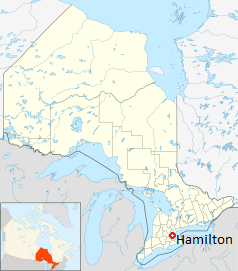
\includegraphics[scale=0.85]{Hamilton.png}
\caption{Położenie Hamilton}\label{fig:Hamilton}
\end{figure}


\begin{figure}[h]
\centering

\includegraphics[scale=0.25]{Herb.png}
\caption{Herb Hamilton}
\end{figure}
\end{document}
\end{document}
